% !TEX root = btstack_gettingstarted.tex

\pagebreak

\section{Protocols}
\label{section:protocols_profiles}

BTstack is a modular dual-mode Bluetooth stack, supporting both the Bluetooth Basic Rate/Enhanced Date Rate (BR/EDR)  as well as the Bluetooth Low Energy LE). The BR/EDR technology, also known as Classic Bluetooth, provides a robust wireless connection between devices designed for high data rate transfer. In contrast, the LE technology has a lower throughput but also lower energy consumption, faster connection setup, and the ability to connect to more device in parallel.

So far, the most popular use of BTstack is in peripheral devices that can be connected via SPP (Android 2.0 or higher) and GATT (Android 4.3 or higher, and iOS 5 or higher). If higher data rates with iOS devices are neccessary, the iAP1 and iAP2 protocols of the Made for iPhone programm can be used. Please contact us directly for information of BTstack and MFi.

Bluetooth devices implement one or more Bluetooth profiles. A Bluetooth profile specifies how one or more Bluetooth protocols are used to achieve its goals. As an example, the Serial Port Profile (SPP) basically specifies that compatible devices should provide a Service Discovery Protocol record that includes the RFCOMM channel to use for the actual communication.

In the following, we first explain how the various Bluetooth protocols are used. In the next chapter, we go over the profiles.																			
% \item Classic Bluetooth applications
% \item Low Energy (LE) Bluetooth applications
% \item Dual-mode applications (using both Classic and LE technologies) 
% \item Made for iPhone applications (MFi)
% \end{itemize}

\begin{figure}[htbp] %  figure placement: here, top, bottom, or page
   \centering
   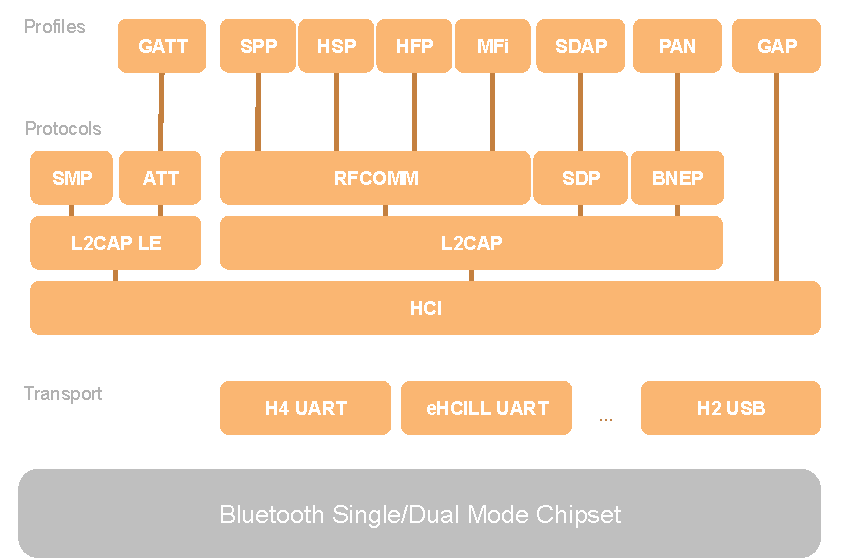
\includegraphics[width=0.9\textwidth]{picts/btstack-protocols.pdf} 
   \caption{BTstack Protocol Architecture}
   \label{fig:BTstackProtocolArchitecture}
\end{figure}

%  As depicted in Figure \ref{fig:BTstackProtocolArchitecture}, BTstack implements following Bluetooth technologies:
% \begin{itemize}
% \item Classic Bluetooth:
% 	\begin{itemize}
% 	\item protocols: HCI, L2CAP, RFCOMM, SDP, BNEP
% 	\item profiles: GAP, SPP, PAN (PAN User (PANU))
% 	\end{itemize}
% \item Bluetooth Low Energy:
% 	\begin{itemize}
% 	\item protocols: HCI, L2CAP-LE, SMP, ATT
% 	\item profiles: GAP-LE, GATT
% 	\end{itemize}
% \end{itemize}

\subsection{HCI - Host Controller Interface}

The HCI protocol provides a command interface to the Bluetooth chipset. In BTstack, the HCI implementation also keeps track of all active connections and also handles the re-assembly of higher layer (L2CAP) packets. Many features of the Generic Access Profile (GAP Classic) can be achieved by sending a single HCI command. Because of this, if there's no special GAP function, please consider sending the HCI command directly, as explained in the following. 

\subsubsection{Defining custom HCI command templates}

Each HCI command is assigned a 2-byte OpCode used to uniquely identify different types of commands. The OpCode parameter is divided into two fields, called the OpCode Group Field (OGF) and OpCode Command Field (OCF), see \BluetoothSpecification{} - Core Version 4.0, Volume 2, Part E, Chapter 5.4. In a HCI command packet, the OpCode is followed by parameter total length, and the actual parameters.

BTstack provides the \emph{hci\_cmd\_t} struct as a compact format to define HCI command packets, see Listing \ref{HCIcmdTemplate},  and \path{include/btstack/hci_cmds.h} file in the source code. The OpCode of a command can be calculated using the OPCODE macro. 


\noindent\begin{minipage}{\textwidth}
\begin{lstlisting}[caption = hci\_cmds.h defines HCI command template., label=HCIcmdTemplate]
// Calculate combined ogf/ocf value.
#define OPCODE(ogf, ocf) (ocf | ogf << 10)

// Compact HCI Command packet description.
typedef struct {
    uint16_t    opcode;
    const char *format;
} hci_cmd_t;

extern const hci_cmd_t hci_write_local_name;
...
\end{lstlisting}
\end{minipage}

\begin{lstlisting}[caption=hci.h defines possible OGFs used for creation of a HCI command., label=hciCmdOGF]
#define OGF_LINK_CONTROL  0x01
#define OGF_LINK_POLICY  0x02
#define OGF_CONTROLLER_BASEBAND  0x03
#define OGF_INFORMATIONAL_PARAMETERS 0x04
#define OGF_LE_CONTROLLER   0x08
#define OGF_BTSTACK  0x3d
#define OGF_VENDOR  0x3f
\end{lstlisting}

Listing \ref{hciCmdOGF} shows the OGFs provided by BTstack in \path{src/hci.h} file.  For all existing Bluetooth commands and their OCFs see \BluetoothSpecificationURL{} - Core Version 4.0, Volume 2, Part E, Chapter 7.

Listing \ref{HCIcmdExample} illustrates the \emph{hci\_write\_local\_name} HCI command template from \mbox{BTstack} library. It uses  OGF\_CONTROLLER\_BASEBAND as OGF, 0x13 as OCF, and has one parameter with format "N" indicating a null terminated UTF-8 string. Table \ref{table:hciformat} lists the format specifiers supported by BTstack. Check \path{src/hci_cmds.c} for other predefined HCI commands and info on their parameters.

\begin{lstlisting}[caption= Example of HCI command template., label=HCIcmdExample]
// Sets local Bluetooth name
const hci_cmd_t hci_write_local_name = {
    OPCODE(OGF_CONTROLLER_BASEBAND, 0x13), "N"
    // Local name (UTF-8, Null Terminated, max 248 octets)
};
\end{lstlisting}

\begin{table*}\centering
\caption{Supported Format Specifiers of HCI Command Parameter}
\begin{tabular}{cl}\toprule
Format Specifier & Description\\ 
\midrule
"1" & 8 bit value \\
"2" & 16 bit value \\
"H" & HCI handle \\
"3" & 24 bit value \\
"4" & 32 bit value \\
"B" & Bluetooth address \\
"D" & 8 byte data block \\
"E" & Extended Inquiry Information 240 octets \\
"N" & UTF8 string, null terminated \\
"P" & 16 byte PIN code or link key \\
"A" & 31 bytes advertising data \\
"S" & Service Record (Data Element Sequence)\\
\bottomrule
\label{table:hciformat}
\end{tabular}
\end{table*}

\subsubsection{Sending  HCI command based on a template}

\begin{lstlisting}[caption= Send hci\_write\_local\_name command that takes a string as a parameter., label=HCIcmdExampleLocalName]
if (hci_can_send_packet_now(HCI_COMMAND_DATA_PACKET)){
    hci_send_cmd(&hci_write_local_name, "BTstack Demo");
}  
\end{lstlisting}

You can use the \emph{hci\_send\_cmd} function to send HCI command based on a template and a list of parameters. However, it is necessary to check that the outgoing packet buffer is empty and that the Bluetooth module is ready to receive the next command - most modern Bluetooth modules only allow  to send a single HCI command. 
This can be done by calling \emph{hci\_can\_send\_command\_packet\_now()} function, which returns true, if it is ok to send.

Listing \ref{HCIcmdExampleLocalName} illustrates how to manually set the device name with the HCI Write Local Name command. 

Please note, that an application rarely has to send HCI commands on its own. Instead, BTstack provides convenience functions in HCI/GAP and higher level protocols use HCI automatically. E.g. to set the name, you can call \emph{gap\_set\_local\_name()} before powering up. The main use of HCI commands in application is during the startup phase to configure special features not available via the GAP API yet.



\subsection{L2CAP -  Logical Link Control and Adaptation Protocol}
The L2CAP protocol supports higher level protocol multiplexing and packet fragmentation. It provides the base for the RFCOMM and BNEP protocols. For all profiles that are officially supported by BTstack, L2CAP does not need to be used directly. For testing or the development of custom protocols, it's helpful to be able to access and provide L2CAP services however.

\subsubsection{Access an L2CAP service on a remote device}
L2CAP is based around the concept of channels. A channel is a logical connection on top of a baseband connection. Each channel is bound to a single protocol in a many-to-one fashion. Multiple channels can be bound to the same protocol, but a channel cannot be bound to multiple protocols. Multiple channels can share the same baseband connection.

\begin{lstlisting}[caption=L2CAP handler for outgoing L2CAP channel.,label=L2CAPremoteService]
btstack_packet_handler_t l2cap_packet_handler;

void btstack_setup(){
    ...
    l2cap_init();
}

void create_outgoing_l2cap_channel(bd_addr_t address, uint16_t psm, uint16_t mtu){
     l2cap_create_channel_internal(NULL, l2cap_packet_handler, remote_bd_addr, psm, mtu);
}

void l2cap_packet_handler(uint8_t packet_type, uint16_t channel, uint8_t *packet, uint16_t size){
    if (packet_type == HCI_EVENT_PACKET &&
          packet[0] == L2CAP_EVENT_CHANNEL_OPENED){
        if (packet[2]) {
            printf("Connection failed\n\r");
            return;
        }
        printf("Connected\n\r");
    }
    if (packet_type == L2CAP_DATA_PACKET){
        // handle L2CAP data packet
        return;
    }
}
\end{lstlisting}

To communicate with an L2CAP service on a remote device, the application on a local Bluetooth device initiates the L2CAP layer using the \emph{l2cap\_init} function, and then creates an outgoing L2CAP channel to the PSM of a remote device using the \emph{l2cap\_create\_channel\_internal} function. The  \emph{l2cap\_-create\_channel\_internal} function will initiate a new baseband connection if it does not already exist. The packet handler that is given as an input parameter of the L2CAP create channel function will be assigned to the new outgoing L2CAP channel. This handler receives the L2CAP\_EVENT\_CHANNEL\_OPENED and L2CAP\_EVENT\_CHAN-NEL\_CLOSED events and L2CAP data packets, as shown in Listing \ref{L2CAPremoteService}.


\subsubsection{Provide an L2CAP service}

To provide an L2CAP service, the application on a local Bluetooth device must init the L2CAP layer and register the service with \emph{l2cap\_register\_service\_internal}. From there on, it can wait for incoming L2CAP connections. The application can accept or deny an incoming connection by calling the \emph{l2cap\_accept\_connection\_internal} and \emph{l2cap\_deny\_connection\_internal} functions respectively. If a connection is accepted and the incoming L2CAP channel gets successfully opened, the L2CAP service can send L2CAP data packets to the connected device with \emph{l2cap\_send\_internal}. 

\begin{lstlisting}[caption=Providing an L2CAP service., label=L2CAPService]
void btstack_setup(){
    ...
    l2cap_init();
    l2cap_register_service_internal(NULL, packet_handler, 0x11,100);
}

void packet_handler (uint8_t packet_type, uint16_t channel, uint8_t *packet, uint16_t size){
      ...
      if (packet_type == L2CAP_DATA_PACKET){
        // handle L2CAP data packet
        return;
    }
    switch(event){
        ...
        case L2CAP_EVENT_INCOMING_CONNECTION:
            bt_flip_addr(event_addr, &packet[2]);
            handle     = READ_BT_16(packet, 8); 
            psm        = READ_BT_16(packet, 10); 
            local_cid  = READ_BT_16(packet, 12); 
            printf("L2CAP incoming connection requested.");
            l2cap_accept_connection_internal(local_cid);
            break;
        case L2CAP_EVENT_CHANNEL_OPENED:
            bt_flip_addr(event_addr, &packet[3]);
            psm = READ_BT_16(packet, 11); 
            local_cid = READ_BT_16(packet, 13); 
            handle = READ_BT_16(packet, 9);
            if (packet[2] == 0) {
                printf("Channel successfully opened.");
            } else {
                printf("L2CAP connection failed. status code.");
            }
            break;        
        case L2CAP_EVENT_CREDITS:
        case DAEMON_EVENT_HCI_PACKET_SENT:
            tryToSend();
            break;
        case L2CAP_EVENT_CHANNEL_CLOSED:
            break;
    }
}
\end{lstlisting}

Sending of L2CAP data packets may fail due to a full internal BTstack outgoing packet buffer, or if the ACL buffers in the Bluetooth module become full, i.e., if the application is sending faster than the packets can be transferred over the air. In such case, the application can try sending again upon reception of DAEMON\_EVENT\_HCI\_PACKET\_SENT or L2CAP\_EVENT\_CREDITS event. The first event signals that the internal BTstack outgoing buffer became free again, the second one signals the same for ACL buffers in the Bluetooth chipset. Listing \ref{L2CAPService} provides L2CAP service example code.

\todo{\textbf{L2CAP and Security Levels}} \\

\subsubsection{L2CAP LE - L2CAP Low Energy Protocol}
In addition to the full L2CAP implementation in the \emph{src} folder, BTstack provides an optimized v\emph{l2cap\_le} implementation in the \emph{ble} folder. This L2CAP LE variant can be used for single-mode devices and provides the base for the ATT and SMP protocols.



\subsection{RFCOMM - Radio Frequency Communication Protocol}
%\label{section:flowcontrol}
The Radio frequency communication (RFCOMM) protocol provides emulation of serial ports over the L2CAP protocol.
and reassembly. It is the base for the Serial Port Profile and other profiles used for telecommunication like Head-Set Profile, Hands-Free Profile, Object Exchange (OBEX) etc.

\subsubsection{RFCOMM flow control.}
RFCOMM has a mandatory credit-based flow-control. This means that two devices that established RFCOMM connection, use credits to keep track of how many more RFCOMM data packets can be sent to each. If a device has no (outgoing) credits left, it cannot send another RFCOMM packet, the transmission must be paused. During the connection establishment, initial credits are provided. BTstack tracks the number of credits in both directions. If no outgoing credits are available, the RFCOMM send function will return an error, and you can try later. For incoming data, BTstack provides channels and services with and without automatic credit management via different functions to create/register them respectively. If the management of credits is automatic, the new credits are provided when needed relying on ACL flow control - this is only useful if there is not much data transmitted and/or only one physical connection is used. If the management of credits is manual, credits are provided by the application such that it can manage its receive buffers explicitly. 

% \todo{\textbf{RFCOMM port configuration for both local and remote}}\\
% \todo{\textbf{RFCOMM  modem and line status control/information}}\\
% \todo{\textbf{RFCOMM\_AGGREGATE\_FLOW\_OFF example}}\\
% \todo{\textbf{RFCOMM and Security Levels}}\\

\subsubsection{Access an RFCOMM service on a remote device}
\label{subsubsection:rfcommlient}

To communicate with an RFCOMM service on a remote device, the application on a local Bluetooth device initiates the RFCOMM layer using the \emph{rfcomm\_init} function, and then creates an outgoing RFCOMM channel to a given server channel on a remote device using the \emph{rfcomm\_create\_channel\_internal} function. The  \emph{rfcomm\_create\_channel\_intern-al} function will initiate a new L2CAP connection for the RFCOMM multiplexer, if it does not already exist. The channel will automatically provide enough credits to the remote side. To provide credits manually, you have to create the RFCOMM connection by calling \emph{rfcomm\_create\_channel\_with\_initial\_credits\_internal} - see Section \ref{sec:manualCredits}.


The packet handler that is given as an input parameter of the RFCOMM create channel function will be assigned to the new outgoing \mbox{RFCOMM} channel. This handler receives the RFCOMM\_EVENT\_OPEN\_CHAN-NEL\_COMPLETE and RFCOMM\_EVENT\_CHANNEL\_CLOSED events, and RFCOMM data packets, as shown in Listing \ref{RFCOMMremoteService}.

\subsubsection{Provide an RFCOMM service}
\label{section:rfcomm_service}

To provide an RFCOMM service, the application on a local Bluetooth device must first init the L2CAP and RFCOMM layers and then register the service with \emph{rfcomm\_register\_service\_internal}. From there on, it can wait for incoming RFCOMM connections. The application can accept or deny an incoming connection by calling the \emph{rfcomm\_accept\_connection-\_internal} and \emph{rfcomm\_deny\_connection\_internal} functions respectively. If a connection is accepted and the incoming RFCOMM channel gets successfully opened, the RFCOMM service can send RFCOMM data packets to the connected device with \emph{rfcomm\_send\_internal} and receive data packets by the packet handler provided by the \emph{rfcomm\_register\_service\_internal} call.

Sending of RFCOMM data packets may fail due to a full internal BTstack outgoing packet buffer, or if the ACL buffers in the Bluetooth module become full, i.e., if the application is sending faster than the packets can be transferred over the air. In such case, the application can try sending again upon reception of DAEMON\_EVENT\_HCI\_PACKET\_SENT or RFCOMM\_EVENT\_CREDITS event. The first event signals that the internal BTstack outgoing buffer became free again, the second one signals that the remote side allowed to send another  packet. Listing \ref{RFCOMMService} provides the RFCOMM service example code.

\begin{lstlisting}[caption= RFCOMM service with automatic credit management. , label=automaticFlowControl]
void btstack_setup(void){
    ...
    // init RFCOMM
    rfcomm_init();
    rfcomm_register_packet_handler(packet_handler);
    rfcomm_register_service_internal(NULL, rfcomm_channel_nr, 100); 
}
\end{lstlisting}


\subsubsection{Living with a single output buffer}
\label{section:single_buffer}
% l2cap checks hci_can_send_packet now
Outgoing packets, both commands and data, are not queued in BTstack. This section explains the consequences of this design decision for sending data and why it is not as bad as it sounds.

\noindent\begin{minipage}{\textwidth}
\begin{lstlisting}[caption=Preparing and sending data., label=SingleOutputBufferTryToSend]
void prepareData(void){
    ...
}

void tryToSend(void){
    if (!dataLen) return;
    if (!rfcomm_channel_id) return;
    
    int err = rfcomm_send_internal(rfcomm_channel_id,  dataBuffer, dataLen);
    switch (err){
        case 0:
            // packet is sent prepare next one
            prepareData();
            break;
        case RFCOMM_NO_OUTGOING_CREDITS:
        case BTSTACK_ACL_BUFFERS_FULL:
            break;
        default:
           printf("rfcomm_send_internal() -> err %d\n\r", err);
        break;
    }
}
\end{lstlisting}
\begin{lstlisting}[ caption= Managing the speed of RFCOMM packet generation., label=SingleOutputBufferTryPH]
void packet_handler (uint8_t packet_type, uint16_t channel, uint8_t *packet, uint16_t size){
    ...
    switch(event){
        case RFCOMM_EVENT_OPEN_CHANNEL_COMPLETE:
            if (status) {
                printf("RFCOMM channel open failed.");
            } else {
                rfcomm_channel_id = READ_BT_16(packet, 12);
                rfcomm_mtu = READ_BT_16(packet, 14);
                printf("RFCOMM channel opened, mtu = %u.", rfcomm_mtu);
            }
            break;
        case RFCOMM_EVENT_CREDITS:
        case DAEMON_EVENT_HCI_PACKET_SENT:
            tryToSend();
            break;
        case RFCOMM_EVENT_CHANNEL_CLOSED:
            rfcomm_channel_id = 0;
            break;
       ...
       }
}
\end{lstlisting}
\end{minipage}

Independent from the number of output buffers, packet generation has to be adapted to the remote receiver and/or maximal link speed. Therefore, a packet can only be generated when it can get sent. With this assumption, the single output buffer design does not impose additional restrictions. In the following, we show how this is used for adapting the RFCOMM send rate. 

BTstack returns BTSTACK\_ACL\_BUFFERS\_FULL, if the outgoing buffer is full and RFCOMM\_NO\_OUTGOING\_CREDITS, if no outgoing credits are available. In Listing \ref{SingleOutputBufferTryToSend}, we show how to resend data packets when credits or outgoing buffers become available.


RFCOMM's mandatory credit-based flow-control imposes an additional constraint on sending a data packet - at least one new RFCOMM credit must be available. BTstack signals the availability of a credit by sending an RFCOMM credit (RFCOMM\_EVENT\_CREDITS) event. 

These two events represent two orthogonal mechanisms that deal with flow control. Taking these mechanisms in account, the application should try to send data packets when one of these two events is received, see Listing \ref{SingleOutputBufferTryPH} for a RFCOMM example.


If the management of credits is manual, credits are provided by the application such that it can manage its receive buffers explicitly, see Listing \ref{explicitFlowControl}.

Manual credit management is recommended when received RFCOMM data cannot be processed immediately. In the SPP flow control example in Section \ref{example:spp_flow_control}, delayed processing of received data is simulated with the help of a periodic timer. To provide new credits, you call the \emph{rfcomm\_grant\_credits} function with the RFCOMM channel ID and the number of credits as shown in Listing \ref{NewCredits}.
Please note that providing single credits effectively reduces the credit-based (sliding window) flow control to a stop-and-wait flow-control that limits the data throughput substantially. On the plus side, it allows for a minimal memory footprint. If possible, multiple RFCOMM buffers should be used to avoid pauses while the sender has to wait for a new credit.


\subsubsection{Slowing down RFCOMM data reception}
\label{sec:manualCredits}
RFCOMM's credit-based flow-control can be used to adapt, i.e., slow down the RFCOMM data to your processing speed. 
For incoming data, BTstack provides channels and services with and without automatic credit management. 
If the management of credits is automatic, see Listing \ref{automaticFlowControl},  new credits are provided when needed relying on ACL flow control. This is only useful if there is not much data transmitted and/or only one physical connection is used


\begin{lstlisting}[float, caption=RFCOMM handler for outgoing RFCOMM channel., label=RFCOMMremoteService] 
void init_rfcomm(){
    ...
    rfcomm_init();
    rfcomm_register_packet_handler(packet_handler);
}

void create_rfcomm_channel(uint8_t packet_type, uint8_t *packet, uint16_t size){
    rfcomm_create_channel_internal(connection, addr, rfcomm_channel);
}

void rfcomm_packet_handler(uint8_t packet_type, uint16_t channel, uint8_t *packet, uint16_t size){
    if (packet_type == HCI_EVENT_PACKET && packet[0] == RFCOMM_EVENT_OPEN_CHANNEL_COMPLETE){
        if (packet[2]) {
            printf("Connection failed\n\r");
            return;
        }
        printf("Connected\n\r");
    }
    
    if (packet_type == RFCOMM_DATA_PACKET){
        // handle RFCOMM data packets
        return;
    }
}
\end{lstlisting}

\begin{lstlisting}[float, caption=Providing RFCOMM service., label=RFCOMMService]
void btstack_setup(){
    ...
    rfcomm_init();
    rfcomm_register_service_internal(NULL, rfcomm_channel_nr, mtu); 
}

void packet_handler(uint8_t packet_type, uint8_t *packet, uint16_t size){
    if (packet_type == RFCOMM_DATA_PACKET){
        // handle RFCOMM data packets
        return;
    }
    ...
    switch (event) {
        ...
        case RFCOMM_EVENT_INCOMING_CONNECTION:
            //data: event(8), len(8), address(48), channel(8), rfcomm_cid(16)
            bt_flip_addr(event_addr, &packet[2]); 
            rfcomm_channel_nr = packet[8];
            rfcomm_channel_id = READ_BT_16(packet, 9);
            rfcomm_accept_connection_internal(rfcomm_channel_id);
            break;
        case RFCOMM_EVENT_OPEN_CHANNEL_COMPLETE:
           // data: event(8), len(8), status (8), address (48), handle(16), server channel(8), rfcomm_cid(16), max frame size(16)
            if (packet[2]) {
                printf("RFCOMM channel open failed.");
                break;
            } 
           // data: event(8), len(8), status (8), address (48), handle (16), server channel(8), rfcomm_cid(16), max frame size(16)
           rfcomm_channel_id = READ_BT_16(packet, 12);
           mtu = READ_BT_16(packet, 14);
           printf("RFCOMM channel open succeeded.");
           break;
        case RFCOMM_EVENT_CREDITS:
        case DAEMON_EVENT_HCI_PACKET_SENT:
            tryToSend();
            break;

        case RFCOMM_EVENT_CHANNEL_CLOSED:
            printf("Channel closed.");
            rfcomm_channel_id = 0;
        break;
    }
}
\end{lstlisting}


% \noindent\begin{minipage}\textwidth
\begin{lstlisting}[ caption= RFCOMM service with manual credit management. , label=explicitFlowControl]
void btstack_setup(void){
    ...
    // init RFCOMM
    rfcomm_init();
    rfcomm_register_packet_handler(packet_handler);
    // reserved channel, mtu=100, 1 credit
    rfcomm_register_service_with_initial_credits_internal(NULL, rfcomm_channel_nr, 100, 1);  
}
\end{lstlisting}

\begin{lstlisting}[caption= Providing new credits , label=NewCredits]
void processing(){
    // process incoming data packet
    ... 
    // provide new credit
    rfcomm_grant_credits(rfcomm_channel_id, 1);
}
\end{lstlisting}

\subsection{SDP - Service Discovery Protocol}
The SDP protocol allows to announce services and discover services provided by a remote Bluetooth device. 

\subsubsection{Create and announce SDP records}
BTstack contains a complete SDP server and allows to register SDP records. An SDP record is a list of SDP Attribute \emph{\{ID, Value\}} pairs that are stored in a Data Element Sequence (DES). The Attribute ID is a 16-bit number, the value can be of other simple types like integers or strings or can itselff contain other DES. 


To create an SDP record for an SPP service, you can call \emph{sdp\_create\_spp\_service} from \path{src/sdp_util.c} with a pointer to a buffer to store the record, the \mbox{RFCOMM} server channel number, and a record name. 

For other types of records, you can use the other functions in \path{src/sdp_util.c}, using the data element \emph{de\_*} functions.  Listing \ref{sdpCreate} shows how an SDP record containing two SDP attributes can be created. First, a DES is created and then the Service Record Handle and Service Class ID List attributes are added to it. The Service Record Handle attribute is added by calling the \emph{de\_add\_number} function twice: the first time to add 0x0000 as attribute ID, and the second time to add the actual record handle (here 0x1000) as attribute value. The Service Class ID List attribute has ID 0x0001, and it requires a list of UUIDs as attribute value. To create the list, \emph{de\_push\_sequence} is called, which "opens" a sub-DES. The returned pointer is used to add elements to this sub-DES. After adding all UUIDs, the sub-DES is "closed" with \emph{de\_pop\_sequence}.

\subsubsection{Query remote SDP service}
\label{subsection:querysdp}

BTstack provides an SDP client to query SDP services of a remote device. The SDP Client API  is shown in Appendix \ref{appendix:api_sdp_client}. The \emph{sdp\_client\_query} function initiates an L2CAP connection to the remote SDP server. Upon connect, a \emph{Service Search Attribute} request with a \emph{Service Search Pattern} and a \emph{Attribute ID List} is sent. The result of the \emph{Service Search Attribute} query contains a list of \emph{Service Records}, and each of them contains the requested attributes. These records are handled by the SDP parser. The parser delivers SDP\_PARSER\_ATTRIBUTE\_VALUE and SDP\_PARSER\_COMPLETE events via a registered callback. The SDP\_PARSER\_ATTRIBUTE\_VALUE event delivers the attribute value byte by byte.

On top of this, you can implement specific SDP queries. For example, BTstack provides a query for RFCOMM service name and channel number. This information is needed, e.g., if you want to connect to a remote SPP service. The query delivers all matching RFCOMM services, including its name and the channel number, as well as a query complete  event via a registered callback, as shown in Listing \ref{SDPClientRFCOMM}.

\begin{lstlisting}[caption=Searching RFCOMM services on a remote device., label=SDPClientRFCOMM ]
bd_addr_t remote = {0x04,0x0C,0xCE,0xE4,0x85,0xD3};

void packet_handler (void * connection, uint8_t packet_type, uint16_t channel, uint8_t *packet, uint16_t size){
    if (packet_type != HCI_EVENT_PACKET) return;

    uint8_t event = packet[0];
    switch (event) {
        case BTSTACK_EVENT_STATE:
            // bt stack activated, get started 
            if (packet[2] == HCI_STATE_WORKING){
            	  sdp_query_rfcomm_channel_and_name_for_uuid(remote, 0x0003);
            }
            break;
        default:
            break;
    }
}

static void btstack_setup(){
   ...
    // init L2CAP
    l2cap_init();
    l2cap_register_packet_handler(packet_handler);
}

void handle_query_rfcomm_event(sdp_query_event_t * event, void * context){
    sdp_query_rfcomm_service_event_t * ve;
            
    switch (event->type){
        case SDP_QUERY_RFCOMM_SERVICE:
            ve = (sdp_query_rfcomm_service_event_t*) event;
            printf("Service name: '%s', RFCOMM port %u\n", ve->service_name, ve->channel_nr);
            break;
        case SDP_QUERY_COMPLETE:
            report_found_services();
            printf("Client query response done with status %d. \n", ce->status);
            break;
    }
}

int main(void){
    hw_setup();
    btstack_setup();
    
    // register callback to receive matching RFCOMM Services and 
    // query complete event 
    sdp_query_rfcomm_register_callback(handle_query_rfcomm_event, NULL);

    // turn on!
    hci_power_control(HCI_POWER_ON);
    // go!
    run_loop_execute(); 
    return 0;
}

\end{lstlisting}

\begin{lstlisting}[caption=Creating record with the data element (\emph{de\_*}) functions., label=sdpCreate]
uint8_t des_buffer[200];
uint8_t* attribute;
de_create_sequence(service);
    
// 0x0000 "Service Record Handle"
de_add_number(des_buffer, DE_UINT, DE_SIZE_16, SDP_ServiceRecordHandle);
de_add_number(des_buffer, DE_UINT, DE_SIZE_32, 0x10001);
    
// 0x0001 "Service Class ID List"
de_add_number(des_buffer,  DE_UINT, DE_SIZE_16, SDP_ServiceClassIDList);
attribute = de_push_sequence(des_buffer);
{
    de_add_number(attribute,  DE_UUID, DE_SIZE_16, 0x1101 );
}
de_pop_sequence(des_buffer, attribute);
\end{lstlisting}
% \end{minipage}

\subsection{BNEP -  Bluetooth Network Encapsulation Protocol}
The BNEP protocol is built on top of L2CAP and it is used to transport control and data packets over standard network protocols such as TCP, IPv4 or IPv6.  BNEP specifies a minimum L2CAP MTU of 1691 bytes. 

To receive BNEP events, please register a packet handler with \emph{bnep\_register\_packet\_handler}.

\subsubsection{Access a BNEP service on a remote device}
To connect to a remote BNEP service, you need to know its UUID. The set of available UUIDs can be queried by a SDP query for the PAN profile. Please see section \ref{section:pan_profile} for details. With the remote UUID, you can create a connection using the \emph{bnep\_connect} function. You'll receive a \emph{BNEP\_EVENT\_OPEN\_CHANNEL\_COMPLETE} on success or failure. 

After the connection was opened successfully, you can send and receive Ethernet packets. Before sending an Ethernet frame with \emph{bnep\_send},   \emph{bnep\_can\_send\_packet\_now} needs to return true. Ethernet frames are received via the registered packet handler with packet type \emph{BNEP\_DATA\_PACKET}.

BTstack BNEP implementation supports both network protocol filter and multicast filters with \emph{bnep\_set\_net\_type\_filter} and \emph{bnep\_set\_multicast\_filter} respectively.

Finally, to close a BNEP connection, you can call \emph{bnep\_disconnect}

\subsubsection{Provide BNEP service}
You can also provide a BNEP service by calling \emph{bnep\_register\_service} with the provided service UUID and a max frame size.

After an incoming connection was established, a \emph{BNEP\_EVENT\_INCOMING\_CONNECTION} event is received. Ethernet packets can now be sent and received as in the previous section.

\subsection{ATT - Attribute Protocol}

The ATT protocol is used by the ATT client to read and write attribute values stored on the ATT server. In addition, the ATT server can notify the client about attribute value changes. An attribute has a handle, a type, and a set of properties.

The GATT profile is built upon ATT and provides higher level organization of the ATT attributes into GATT Services and GATT Characteristics. In BTstack, the complete ATT client functionality is included within the GATT Client. On the server side, one ore more GATT profiles are converted ahead of time into the corresponding ATT attribute database and provided by the \emph{att\_server} implementation. While constant data is automatically served, dynamic data can be queried from the application. In addition, notifications and indications can be sent. Please see section \ref{section:GATT} for more.

\subsection{SMP - Security Manager Protocol }

The SMP protocol allows to setup authenticated and encrypted LE connection. After initialization and configuration, SMP handles security related functions on it's own but emits events when feedback from the main app or even the user is required. The two main tasks of the SMP are: bonding and identity resolving.

\subsubsection{Initialization}

To activate the security manager, call \emph{sm\_init()}. 

If you're creating a product, you should also call \emph{sm\_set\_ir()} and \emph{sm\_set\_er()} with a fixed random 16 byte number. If possible use a unique random number per device instead of deriving it from the product serial number something similar. The encryption key generated by the BLE peripheral ultimately will be derived from the ER key seed. See Blueooth Core V4.0, Vol 3, Part G, 5.2.2 for more details on deriving the different keys. The IR key is used to identify a device if private, resolvable Bluetooth addresses are used.

\subsubsection{Configuration}

To receive events from the Security Manager, a call back is neccessary. How to register this packet handler depends on your application configuration. 

When \emph{att\_server.c} is used to provide a GATT/ATT service, \emph{att\_server.c} registers itself as the Security Manager packet handler. Security Manager events are then are received by the application via the \emph{att\_server} packet handler.

If \emph{att\_server} is not used, you can directly register your packet handler with the security manager. 

The default Security Manager configuration in BTstack is to be as open as possible: accept all Short Term Key (STK) Generation methods, accepted encryption key size from 7..16 bytes, and no authentication requirements. The default IO Capabilities are \emph{IO\_CAPABILITY\_NO\_INPUT\_NO\_OUTPUT}.

To configure the bonding options, you can use the following functions:
\begin{itemize}
\item \emph{sm\_set\_accepted\_stk\_generation\_methods}
\item \emph{sm\_set\_encryption\_key\_size\_range}
\item \emph{sm\_set\_authentication\_requirements}
\item \emph{sm\_set\_io\_capabilities}
\end{itemize}

\subsubsection{Identity Resolving}

Identity resolving is the process of matching a private, resolvable Bluetooth address to a previously paired device using its Identity Resolving (IR) key. For this, each device in the le central device db needs to get compared to the device address in question. After an LE connection gets established, BTstack automatically tries to resolve the address of this device. During this lookup, BTstack first emits the \emph{SM\_IDENTITY\_RESOLVING\_STARTED} event and later \emph{SM\_IDENTITY\_RESOLVING\_SUCCEEDED} or \emph{SM\_IDENTITY\_RESOLVING\_FAILED}.

\subsubsection{Bonding process}

In Bluetooth LE, there are thee main methods of establishing a first encrypted connection. From most secure to least secure, these are: Out-of-Band (OOB) Data , Passkey, and Just Works.

With OOB data, there needs to be a pre-shared secret 16 byte key. In most cases, this is not an option, especially since popular OS like iOS don't provide a way to specify it. It some applications, where both sides of a Bluetooth link are developed together, this could provide a viable option.

To provide OOB data, you can register an OOB data callback with \emph{sm\_register\_oob\_data\_callback}. 

Depending on the authentication requirements, available OOB data, and the enabled STK generation methods, BTstack will request feedback from the app in the form of an event:
\begin{itemize}
\item \emph{SM\_PASSKEY\_INPUT\_NUMBER}: request user to input a passkey
\item \emph{SM\_PASSKEY\_DISPLAY\_NUMBER}: show a passkey to the user
\item \emph{SM\_JUST\_WORKS\_REQUEST}: request a user to accept a Just Works pairing
\end{itemize}

If the user stops the bonding process, \emph{sm\_bonding\_decline} should be called. Otherwise, \emph{sm\_just\_works\_confirm} or \emph{sm\_passkey\_input} can be called.

After the bonding process, \emph{SM\_PASSKEY\_DISPLAY\_CANCEL} is emitted to update the user interface.

% /subsubsection {Authorization}
% SM_AUTHORIZATION_REQUEST
% SM_AUTHORIZATION_RESULT

% ------

\section{Profiles}
As promised in the previous chapter, we explain how to implement various Bluetooth profiles in this one.


\subsection{GAP - Generic Access Profile: Classic}
The GAP profile defines how device find each other and establish a secure connection for other profiles.
As mentioned before GAP functionality is split between gaph.h and hci.h. Please check both.

\subsubsection{Become discoverable}
A remote unconnected Bluetooth device must be set as "discoverable" in order to be seen by a device performing the inquiry scan. To become discoverable, an application can call \emph{hci\_discoverable\_control}  with input parameter 1. If you want to provide a helpful name for your device, the application can set its local name by sending the $hci\_write\_local\_name$ command. To save energy, you may set the device as undiscoverable again, once a connection is established. See Listing \ref{Discoverable} for an example.

\begin{lstlisting}[caption=Setting device as discoverable. OFF by default., label=Discoverable]
int main(void){
    ... 
    // make discoverable
    hci_discoverable_control(1);
    run_loop_execute(); 
    return 0;
}
void packet_handler (uint8_t packet_type, uint8_t *packet, uint16_t size){
     ...
     switch(state){
          case W4_CHANNEL_COMPLETE:
              // if connection is successful, make device undiscoverable
              hci_discoverable_control(0);
          ...
     }
 }
\end{lstlisting}


\subsubsection{Discover remote devices}
\label{section:DiscoverDevices}
To scan for remote devices, the \emph{hci\_inquiry} command is used. After that, the Bluetooth devices actively scans for other devices and reports these as part of HCI\_EVENT\_INQUIRY\_RESULT, HCI\_EVENT-\_INQUIRY\_RESULT\_WITH\_RSSI, or HCI\_EVENT\_EXTENDED\_INQUIRY\_RE-SPONSE events. Each response contains at least the Bluetooth address, the class of device, the page scan repetition mode, and the clock offset of found device. The latter events add information about the received signal strength or provide the Extended Inquiry Result (EIR). A code snippet is shown in Listing \ref{DiscoverDevices}.

By default, neither RSSI values nor EIR are reported. If the Bluetooth device implements Bluetooth Specification 2.1 or higher, the \emph{hci\_write\_inquiry\_mode} command enables reporting of this advanced features (0 for standard results, 1 for RSSI, 2 for RSSI and EIR). 

A complete GAP inquiry example is provided in Section \ref{example:GapInquiry}.

\begin{lstlisting}[float, caption=Discovering remote Bluetooth devices., label=DiscoverDevices]
void print_inquiry_results(uint8_t *packet){
    int event = packet[0];
    int numResponses = packet[2];
    uint16_t classOfDevice, clockOffset;
    uint8_t  rssi, pageScanRepetitionMode;
    for (i=0; i<numResponses; i++){
        bt_flip_addr(addr, &packet[3+i*6]);
        pageScanRepetitionMode = packet [3 + numResponses*6 + i];
        if (event == HCI_EVENT_INQUIRY_RESULT){
            classOfDevice = READ_BT_24(packet, 3 + numResponses*(6+1+1+1) + i*3);
            clockOffset =   READ_BT_16(packet, 3 + numResponses*(6+1+1+1+3) + i*2) & 0x7fff;
            rssi  = 0;
        } else {
            classOfDevice = READ_BT_24(packet, 3 + numResponses*(6+1+1)     + i*3);
            clockOffset =   READ_BT_16(packet, 3 + numResponses*(6+1+1+3)   + i*2) & 0x7fff;
            rssi  = packet [3 + numResponses*(6+1+1+3+2) + i*1];
        }
        printf("Device found: %s with COD: 0x%06x, pageScan %u, clock offset 0x%04x, rssi 0x%02x\n", bd_addr_to_str(addr), classOfDevice, pageScanRepetitionMode, clockOffset, rssi);
    }
}

void packet_handler (uint8_t packet_type, uint8_t *packet, uint16_t size){
    ...
    switch (event) {
         case HCI_STATE_WORKING:
            hci_send_cmd(&hci_write_inquiry_mode, 0x01); // with RSSI
            break;
        case HCI_EVENT_COMMAND_COMPLETE:
            if (COMMAND_COMPLETE_EVENT(packet, hci_write_inquiry_mode) ) {
                start_scan();
            }
        case HCI_EVENT_COMMAND_STATUS:
            if (COMMAND_STATUS_EVENT(packet, hci_write_inquiry_mode) ) {
                printf("Ignoring error (0x%x) from hci_write_inquiry_mode.\n", packet[2]);
                hci_send_cmd(&hci_inquiry, HCI_INQUIRY_LAP, INQUIRY_INTERVAL, 0);
            }
            break;
        case HCI_EVENT_INQUIRY_RESULT:
        case HCI_EVENT_INQUIRY_RESULT_WITH_RSSI:
            print_inquiry_results(packet);
            break;
       ...
    }
}
\end{lstlisting}

\begin{lstlisting}[caption=Answering authentication request with PIN 0000., label=PinCodeRequest]
void packet_handler (uint8_t packet_type, uint8_t *packet, uint16_t size){
    ...
    switch (event) {
        case HCI_EVENT_PIN_CODE_REQUEST:
            // inform about pin code request
            printf("Pin code request - using '0000'\n\r");
            bt_flip_addr(bd_addr, &packet[2]);
            
            // baseband address, pin length, PIN: c-string
            hci_send_cmd(&hci_pin_code_request_reply, &bd_addr, 4, "0000");
            break;
       ...
    }
}
\end{lstlisting}

\subsubsection{Pairing of Devices}
By default, Bluetooth communication is not authenticated, and any device can talk to any other device. A Bluetooth device (for example, cellular phone) may choose to require authentication to provide a particular service (for example, a Dial-Up service). The process of establishing authentication is called pairing. Bluetooth provides two mechanism for this.

On Bluetooth devices that conform to the Bluetooth v2.0 or older specification, a PIN code (up to 16 bytes ASCII) has to be entered on both sides. This isn't optimal for embedded systems that do not have full I/O capabilities. To support pairing with older devices using a PIN, see Listing \ref{PinCodeRequest}.

The Bluetooth v2.1 specification introduces Secure Simple Pairing (SSP), which is a better approach as it both improves security and is better adapted to embedded system. With SSP, the devices first exchange their IO Capabilities and then settle on one of several ways to verify that the pairing is legitimate. If the Bluetooth device supports SSP, BTstack enables it by default and even automatically accepts SSP pairing requests. Depending on the product in which BTstack is used, this may not be desired and should be replaced with code to interact with the user.

Regardless of the authentication mechanism (PIN/SSP), on success, both devices will generate a link key. The link key can be stored either in the Bluetooth module itself or in a persistent storage, see Section \ref{section:persistent_storage}. The next time the device connect and request an authenticated connection, both devices can use the previously generated link key. Please note that the pairing must be repeated if the link key is lost by one device.

\subsubsection{Dedicated Bonding}
Aside from the regular bonding as needed, Bluetooth also provides the concecpt of "dedicated bonding", where a connection is established for the sole purpose of bonding the device. After the bonding process is over, the connection will automatically be terminated. BTstack supports dedicated bonding via the \emph{gap\_dedicated\_bonding} function.

\subsection{SPP - Serial Port Profile}
The SPP profile defines how to set up virtual serial ports and connect two Bluetooth enabled devices. 
%See Appendix \ref{appendix:api_} for the SPP API.
\subsubsection{Providing an SPP Server}
To provide an SPP Server, you need to provide an RFCOMM service with a specific RFCOMM channel number as explained in section \ref{section:rfcomm_service}. Then, you need to create an SDP record for it and publish it with the SDP server. BTstack provides the \emph{sdp\_create\_spp\_service} function in \emph{sdp\_utils.c} that one requires an empyut buffer of approx. 200 bytes, the service channel number, and a service name. Have a look at the SPP Counter example in section \ref{section:sppcounter}.

\subsubsection{Accessing an SPP Server on a remote device}
To access a remote SPP server, you first need to query the remote device for its SPP services. Section \ref{subsection:querysdp} shows how to query for all RFCOMM channels. For SPP, you can do the same but use the SPP UUID 0x1101 for the query. After you have identified the correct RFCOMM channel, you can create an RFCOMM connection as shown in section \ref{subsubsection:rfcommlient}

\subsection{PAN -  Personal Area Networking Profile}
\label{section:pan_profile}
The PAN profile uses BNEP to provide on-demand networking capabilities between Bluetooth devices. The PAN profile defines the following roles:
\begin{itemize}
\item PAN User (PANU)
\item Network Access Point (NAP)
\item Group Ad-hoc Network (GN)
\end{itemize}

PANU is a Bluetooth device that communicates as a client with GN, or NAP, or with another PANU Bluetooth device, through a point-to-point connection. Either the PANU or the other Bluetooth device may terminate the connection at anytime.

NAP is a Bluetooth device that provides the service of routing network packets between PANU by using BNEP and the IP routing mechanism. A NAP can also act as a bridge between Bluetooth networks and other network technologies by using the Ethernet packets.

The GN role enables two or more PANUs to interact with each other through a wireless network without using additional networking hardware. The devices are connected in a piconet where the GN acts as a master and communicates either point-to-point or a point-to-multipoint with a maximum of seven PANU slaves by using BNEP.

Currently, BTstack supports only PANU.

\subsection{GAP - Generic Access Profile: Low Energy}
The GAP profile defines how to discover and how to connect to a Bluetooth device. There are several GAP roles that a Bluetooth device can take, but the most important ones are the Central and the Peripheral role. Peripheral devices are those that provide information or can be controlled and central devices are those that consume information or control the peripherals. Before the connection can be established, devices are first going through the advertising process. What happens with the peripheral device after the central device connect to a it, depends on the peripheral's Bluetooth controller. The peripheral will either stop advertising itself and other devices will no longer be able to see it or connect to it until the existing connection is broken, or it will be able to continue with advertising so that the parallel connections can be established.

% \subsection{Low Energy}
The focus is on two different device roles:  devices that provide services and/or can be controlled and devices that consume services and/or control other devices. Devices are first going through the advertising process that is governed by the Generic Access Profile (GAP). Once the connection is established, the communication will be governed by the Generic Attribute Profile (GATT). Both profiles, GAP and GATT, have concepts that describe these two BLE roles:  GAP defines Peripheral and Central, and GATT defines Server and Client role respectively. The GATT roles are not necessarily tied to specific GAP roles and may be specified by higher layer profiles. GATT is built on top of the Attribute Protocol (ATT), which defines how to discover, read, and write attributes on a peer device. In addition, BLE uses two more BT protocols: SMP for for pairing and transport specific key distribution and L2CAP LE variant optimized for connectionless data used by Bluetooth Low Energy devices. 

\textbf{Private/random addresses.}
To better protect privacy, a LE device can choose use a private i.e. random Bluetooth address. This address changes at a user-specified rate. To allow for later reconnection, the central and peripheral devices exchange their Identity Resolving Keys (IRKs) during bonding. The IRK is used to verify if a new address belongs to a previously bonded device.

\textbf{GAP BLE Roles.}
There are four GAP roles defined for a Bluetooth low energy device: Broadcaster, Observer, Peripheral and Central. A device may operate in multiple GAP roles concurrently.
\begin{itemize}
\item \emph{GAP Broadcaster Role} - A broadcast device only sends advertisements and cannot be connected. It can emit some useful data as part of the advertisement. The most prominent use for this is Apple's iBeacon technology which uses broadcast devices to emit a unique ID. Apple's iOS framework then help to map this ID onto a specific location, e.g., in a museum. Broadcasting is efficient as no connection and no ATT database are needed. To control energy consumption the broadcast interval can be configured. An advertisement can contain up to 31 bytes of information. In addition, another 31 bytes of information can be sent in the scan response.
\item \emph{GAP Observer Role} - An observer device only receives advertising events and cannot be connected. 
\item \emph{GAP Central Role} - The role of the central device is to scan for peripherals, connect to them, and discover and receive data from them or sends data to control them. During scanning the central device can retrieve information on other device such are its name and unique number, as well as some broadcast data from its services. Upon connection, the central explores the device by discovering its primary and included services, characteristics, and characteristic descriptors.
\item \emph{GAP Peripheral Role} - The role of a peripheral device is to deliver information on their inputs, i.e. sensor values, battery level, current time, to the applications running on central devices. It can also receive a write request from a central device and control connected actors, e.g. turn on and set the color of the light. Peripherals can broadcast data, they can be discovered and connected to by a central device, they can stay also disconnected and then establish connection when needed. 
\end{itemize} 

\textbf{Advertising and Scan Response Data.}
There are two ways to send advertising out with GAP: The Advertising Data payload and the Scan Response payload. Both payloads are identical and can contain up to 31 bytes of data, but only the advertising data payload is mandatory. The scan response payload is an optional secondary payload that central devices can request.

\todo{\textbf{Explain how to setup ATT Database}} \\

\subsection{GATT - Generic Attribute Profile}
The GATT profile uses the ATT for discovering services, and for reading and writing characteristic values on a peer device. GATT also specifies the format of data contained on the GATT server: it groups ATT attributes into Services and Characteristics, and defines set of queries the GATT Client can use to discover services, characteristics.

\textbf{GATT LE Roles.}
There are two GATT roles defined for a Bluetooth low energy device:
\begin{itemize}
\item \emph{GATT Server Role} - The GATT server stores the data and accepts GATT client requests, commands and confirmations. The GATT server sends responses to requests and when configured, sends indication and notifications asynchronously to the GATT client. 
\item \emph{GATT Client Role} - The GATT Client is used to discover services, and their characteristics and descriptors on a peer device. It can also subscribe for notifications or indications that the characteristic on the GATT server has changed its value. 
\end{itemize}

\textbf{Attribute Database - GATT-based Profile Hierarchy.}
Attributes, as transported by the Attribute Protocol, are formatted as services and characteristics. Services may contain a collection of characteristics. Characteristics contain a single value and any number of descriptors describing the characteristic value. The peripheral device server (ATT server) provides a set of attributes that are stored in a simple lookup database. GATT formats these attributes as services and characteristics. Services may contain a collection of characteristics. Characteristics contain a single value and any number of descriptors describing the characteristic value. A service starts with a service declaration attribute defining its type, i.e. primary or secondary. It is followed by the included services and characteristics. By means of including services, the service can incorporate more complex behavior, and still keep the definition small. A characteristic is assigned to a single value that can be accessed. It is composed of three basic elements: declaration, value and descriptors. The characteristic declaration defines how the data can be accessed. A characteristic descriptor is used to capture the additional properties, e.g., to configure if the characteristic value should be reported upon its change. Together, characteristic declaration and the descriptors define types of action that can be performed on characteristic value.

The security that is required to access a service or a characteristic is defined in ATT database along with service/characteristic declaration. The GATT Server usually does not initiate any security request, but it can. 


